% Problem and Data Description -- handbook section 3

\subsection{Problem formulation}
\label{subsec:problem-and-data-1}
% Required: Real-world motivation; input; output; prediction unit; mathematical formulation when appropriate; main difficulties.

A vehicle that plans its own path must know not merely that a road is ahead but exactly where the
road ends, where the pavement begins and which pixels belong to a pedestrian. Semantic
segmentation supplies that map, and it is the perception layer beneath driver assistance, road
survey and scene understanding. Cityscapes \cite{cordts2016cityscapes} is the reference benchmark
for the urban case, finely annotated at a resolution high enough that thin structures survive.

The task is dense per-pixel classification and the prediction unit is one pixel, so a single
$512 \times 1024$ frame carries $524{,}288$ predictions. The input is an RGB image
$x \in \mathbb{R}^{3 \times H \times W}$ and the output a label map
$\hat{y} \in \{0, \dots, C-1\}^{H \times W}$ over $C = 19$ evaluated classes. Every model
implements a function $f_\theta$ returning per-pixel logits
$z = f_\theta(x) \in \mathbb{R}^{C \times H \times W}$, and the prediction at pixel $(i,j)$ is
$\hat{y}_{ij} = \arg\max_{c} z_{cij}$. Training minimises the cross-entropy of
Equation~\ref{eq:cross-entropy}, averaged over the pixels that carry an evaluated label:

\begin{equation}
    \mathcal{L}(\theta) = -\frac{1}{|\Omega|} \sum_{(i,j) \in \Omega}
    \log \frac{\exp(z_{y_{ij} i j})}{\sum_{c=1}^{C} \exp(z_{cij})},
    \qquad
    \Omega = \{(i,j) : y_{ij} \neq 255\}.
    \label{eq:cross-entropy}
\end{equation}

The restriction to $\Omega$ is material rather than formal. Section~\ref{subsec:problem-and-data-3} measures
$11.8\%$ of all pixels as unlabelled, and a loss that scored them would train the network to
reproduce the bonnet of the recording vehicle.

Three difficulties dominate, and all three are properties of the data rather than of the
objective. The classes span almost three orders of magnitude in pixel share, so an objective
that weights pixels equally is governed by whatever covers the most ground. Scarcity arrives in
two forms that fail for different reasons, quantified in
Section~\ref{subsec:problem-and-data-3}, and no single remedy addresses both. And the output must
retain spatial resolution: a classifier may collapse the image to a vector, whereas here the
network has to carry location all the way to the prediction, which is what makes the decoder, or
the dilated backbone that replaces it, the architectural question.

\subsection{Dataset description}
\label{subsec:problem-and-data-2}
% Required: Source, version, license; collection and labeling process if known; sample counts and annotations; class or target distribution; storage size and formats; bias and limitations.

Cityscapes \cite{cordts2016cityscapes} is distributed by its authors at
\url{https://www.cityscapes-dataset.com} under a licence permitting non-commercial research and
educational use, and requires a registered account. The two packages used here,
\texttt{leftImg8bit\_trainvaltest} and \texttt{gtFine\_trainvaltest}, were fetched on 7 October
2026. The frames were recorded from a moving vehicle across 27 cities in Germany, France and
Switzerland, over several months, in daylight and fair weather. The fine annotations were drawn
as per-pixel polygons by human annotators and quality-controlled by the dataset authors, so the
labels are expert rather than crowd-sourced.

The fine-annotation set holds $5{,}000$ frames at $1024 \times 2048$: $2{,}975$ in the official
train split across 18 cities, $500$ in val across 3, and $1{,}525$ in test across 6 whose labels
are withheld for the public leaderboard. Images are 8-bit PNG, label maps single-channel PNG of
label ids. Storage is 11~GB of images and 808~MB of labels, from 11.3~GB of archives that can be
deleted once unpacked.

The annotation defines 34 label ids of which 19 are evaluated; the remainder, including void
regions, the ego vehicle and the rectification border, map to the ignore label $255$. The 19
evaluated classes are road, sidewalk, building, wall, fence, pole, traffic light, traffic sign,
vegetation, terrain, sky, person, rider, car, truck, bus, train, motorcycle and bicycle, and
their distribution is the subject of Section~\ref{subsec:problem-and-data-3}.

Three limitations bound what these results can claim. The recording conditions are narrow:
daylight, fair weather, European cities and one camera, so neither the ranking nor the error
structure should be assumed to hold at night, in rain or on another continent. The class
taxonomy embeds decisions that are conventions rather than visual facts, the boundary between
terrain and vegetation among them, so part of the residual error is irreducible. And the ignore
label is not uniformly distributed: $7.7\%$ of every frame is unusable regardless of content,
because the bonnet occupies the bottom and the rectification border the edges, which removes
image area exactly where the road surface nearest the vehicle would be.

\subsection{Exploratory data analysis}
\label{subsec:problem-and-data-3}
% Required: Task-appropriate analysis; the assignment chapter lists the required items.
% Also required: Section 22, segmentation: pixel distribution, region size, and mask quality.

Every measurement in this section is taken over all $2{,}406$ label maps of the
training partition rather than a sample.
Figure~\ref{fig:samples} shows three frames with their annotations.

\begin{figure}[H]
    \centering
    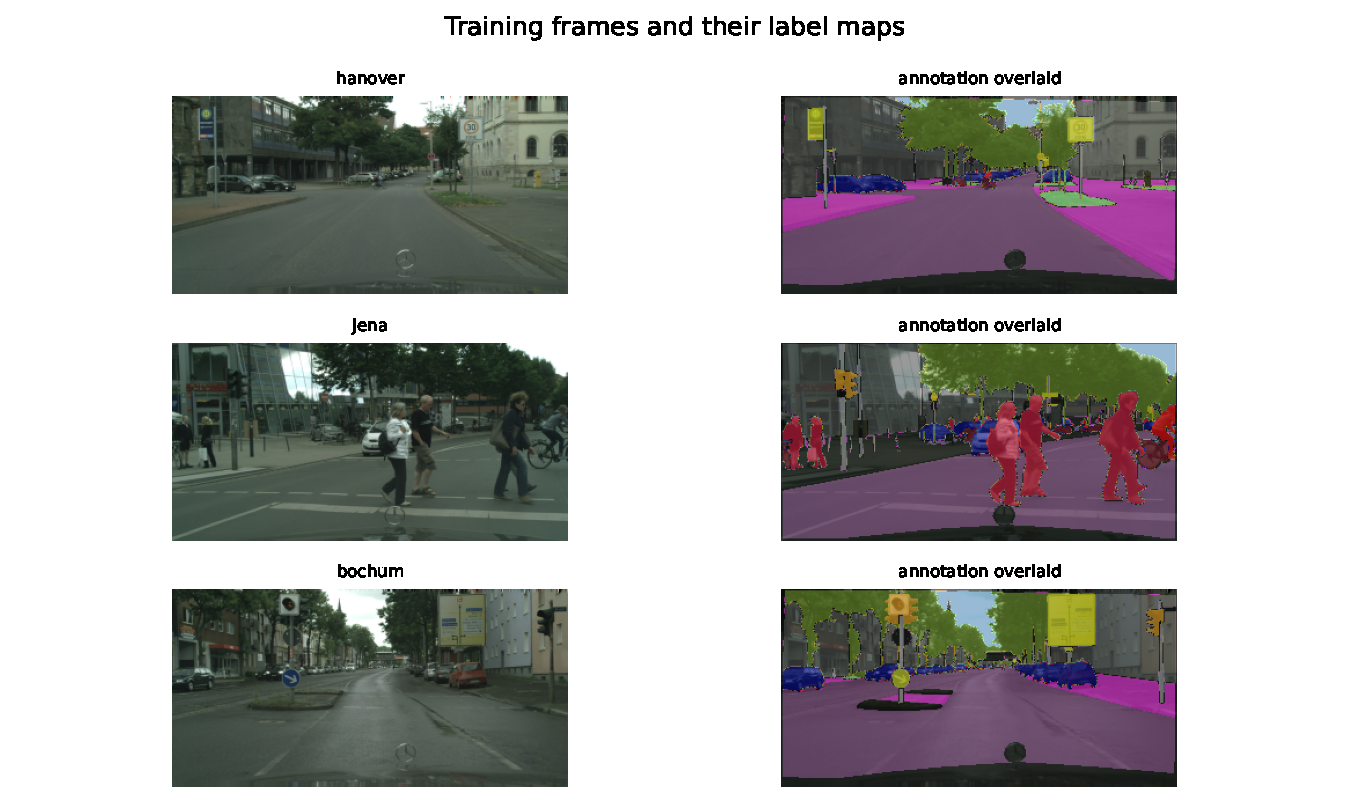
\includegraphics[width=\textwidth]{images/samples.pdf}
    \caption{Training frames and their label maps; dark regions carry the ignore label.}
    \label{fig:samples}
\end{figure}

\textbf{Mask quality.} The annotations are complete in the sense that matters: every frame has a
label map of identical resolution, every pixel carries a valid label id, and no frame was
discarded. What varies is how much of each frame is evaluable. $11.8\%$ of all pixels carry the
ignore label, of which $7.7\%$ is the structural loss described above and the remainder genuine
void annotation. No interpolation is ever applied to a label map, for the reason given in
Section~\ref{subsec:problem-and-data-5}.

\textbf{Pixel distribution.} Table~\ref{tab:class-distribution} and Figure~\ref{fig:classes}
report the distribution three ways, because the mean pixel share alone is misleading. Road,
building and vegetation together occupy $75.8\%$ of evaluated pixels, so a model that predicted
nothing but those three would already reach roughly $0.76$ pixel accuracy. This is the measured
reason mIoU is the primary metric and pixel accuracy decides nothing: mIoU averages over classes,
so the sixteen remaining classes cannot be hidden by the three largest.

\begin{table}[H]
\centering
\caption{Class distribution over the training partition.}
\label{tab:class-distribution}
\small
\begin{tabular}{lrrrr|lrrrr}
\hline
\textbf{Class} & \textbf{Pixels} & \textbf{Images} & \textbf{Area} & \textbf{Crops} &
\textbf{Class} & \textbf{Pixels} & \textbf{Images} & \textbf{Area} & \textbf{Crops} \\
\hline
road       & 36.80\% & 98\% & 33.56\% & 93\% & wall          & 0.74\% & 36\% & 0.69\% & 17\% \\
building   & 22.92\% & 99\% & 20.16\% & 82\% & traffic sign  & 0.56\% & 94\% & 0.31\% & 47\% \\
vegetation & 16.07\% & 97\% & 13.15\% & 71\% & bicycle       & 0.39\% & 54\% & 0.23\% & 26\% \\
car        &  6.78\% & 95\% &  4.18\% & 71\% & truck         & 0.31\% & 12\% & 0.45\% &  4\% \\
sidewalk   &  6.16\% & 94\% &  4.67\% & 79\% & bus           & 0.22\% &  9\% & 0.66\% &  4\% \\
sky        &  3.88\% & 90\% &  2.97\% & 25\% & train         & 0.21\% &  4\% & 0.91\% &  2\% \\
person     &  1.32\% & 79\% &  0.52\% & 46\% & traffic light & 0.20\% & 54\% & 0.18\% & 23\% \\
pole       &  1.17\% & 99\% &  0.83\% & 77\% & rider         & 0.13\% & 33\% & 0.13\% & 13\% \\
terrain    &  1.12\% & 55\% &  0.60\% & 30\% & motorcycle    & 0.11\% & 18\% & 0.13\% &  6\% \\
fence      &  0.92\% & 43\% &  0.81\% & 19\% &               &        &      &        &      \\
\hline
\end{tabular}
\end{table}

\begin{figure}[H]
    \centering
    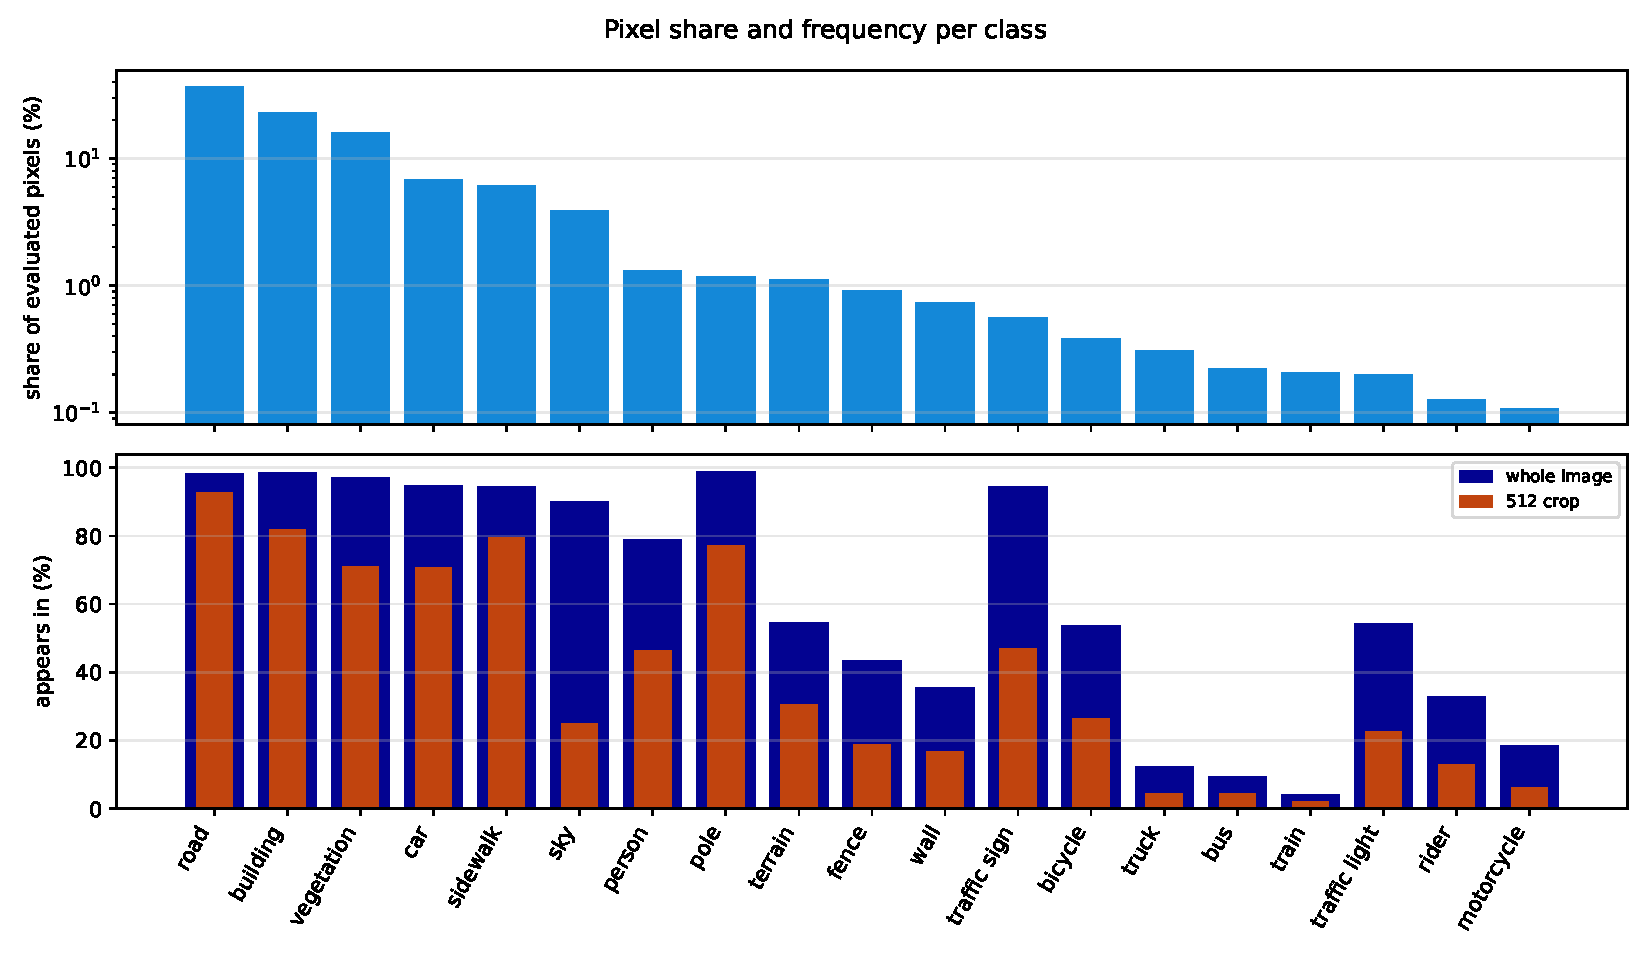
\includegraphics[width=\textwidth]{images/class_distribution.pdf}
    \caption{Pixel share and frequency per class.}
    \label{fig:classes}
\end{figure}

\textbf{Region size, and the two forms of scarcity.} Comparing the \emph{pixels} and
\emph{images} columns of Table~\ref{tab:class-distribution} separates two failure modes that a
single frequency count conflates.

The first is thin structures. Poles account for $1.17\%$ of evaluated pixels but appear in
$99\%$ of images, and traffic signs for $0.56\%$ of pixels in $94\%$ of images. Examples are
therefore abundant; what is scarce is pixel coverage, so the errors these classes produce are
boundary errors rather than the result of too few training instances.

The second is large objects that are seldom photographed. Trains occupy $0.21\%$ of pixels in
$4\%$ of images and buses $0.22\%$ in $9\%$. When one is present, however, its median area is
$0.91\%$ and $0.66\%$ of the frame, four and three times its average share. A reweighted loss addresses the second form and not the first, which is what makes the loss
ablation of Section~\ref{subsec:results-6} worth running.

\textbf{What cropping does to the prior.} The last column of
Table~\ref{tab:class-distribution} samples one random $512 \times 512$ crop per image, which is
what a training batch actually sees. A crop covers an eighth of the resized frame, and it
sharpens the second form of scarcity: trains fall from $4\%$ of images to $2\%$ of crops and
buses from $9\%$ to $4\%$. Sky is the clearest case and is not a rare class at all, falling from
$90\%$ of images to $25\%$ of crops, because it occupies a band at the top of the frame rather
than a compact region. Cropping therefore reshapes the class prior spatially and not only by
area, and the effective training distribution is the crop column rather than the pixel column.

Figure~\ref{fig:cities} completes the picture across the split unit, showing that no city is
large enough to dominate the partition it belongs to.

\begin{figure}[H]
    \centering
    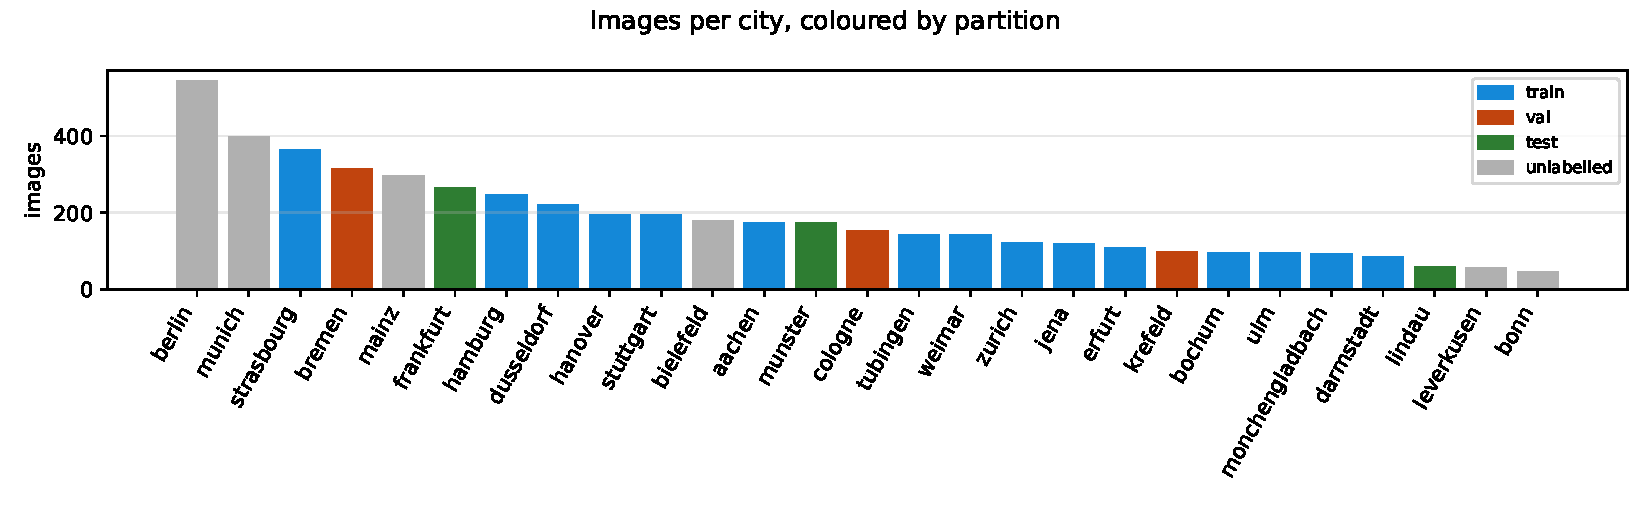
\includegraphics[width=0.9\textwidth]{images/cities.pdf}
    \caption{Frames per city, coloured by partition.}
    \label{fig:cities}
\end{figure}

\subsection{Data splitting}
\label{subsec:problem-and-data-4}
% Required: Train, validation and test; official or custom split; seed; stratification; split unit; leakage prevention; subset selection rules if any.

\textbf{The split unit is the city}, not the frame. Consecutive frames from one street share
buildings, parked cars and road surface, so splitting by frame would place near-duplicates on
both sides of the boundary and let a model score by recognising a scene it had trained on. The
official Cityscapes partitions already share no city, and the split used here preserves that
property.

The official test labels are withheld, so the official validation partition serves as the test set.
A checkpoint cannot then be selected on it without selecting on the test set, so the three
cities that select the checkpoint are held out of the official train partition instead.
Table~\ref{tab:splits} gives the result.

\begin{table}[H]
\centering
\caption{Split sizes.}
\label{tab:splits}
\begin{tabular}{llrr}
\hline
\textbf{Partition} & \textbf{Source} & \textbf{Cities} & \textbf{Images} \\
\hline
Train      & official train                      & 15 & 2{,}406 \\
Validation & official train, held out at seed $0$ &  3 &   569 \\
Test       & official val                        &  3 &   500 \\
\hline
\end{tabular}
\end{table}

Seed $0$ holds out Bremen, Cologne and Krefeld for validation; the test cities are Frankfurt,
Lindau and Münster, as the official partition fixes them. No stratification is applied, because
the unit is a city and every city contains every common class;
Figure~\ref{fig:cities} shows the resulting sizes are comparable. There are no subset selection
rules: the full fine-annotation set is used.

The split is generated once, committed as a file, and read by every run, so it is identical
across models, seeds and machines. Three rules prevent leakage,
each closing a different route. The split file is read rather than regenerated, so no run can
silently resample it. Normalization statistics never come from the data a model is scored on,
as Section~\ref{subsec:problem-and-data-5} describes. And the test partition is read once per
configuration, after model selection concludes, so it never participates in a decision;
Section~\ref{subsec:results-2} reports both splits and the gap between them.

\subsection{Preprocessing}
\label{subsec:problem-and-data-5}
% Required: Cleaning; resize, normalization, tokenization, padding; augmentation; invalid annotation handling; input tensor shapes; one example batch after preprocessing.

No cleaning is required: every frame has a complete label map, and the dataset's own
documentation records no invalid annotations. Invalid and unevaluated content is handled by the
label mapping rather than by discarding data. The 34 label ids are remapped to the 19 train ids
with everything else sent to the ignore label, and that table was read from the dataset's own
toolkit rather than retyped, since a single misplaced row would corrupt every metric in this
report without raising an error.

Images are resized from $1024 \times 2048$ to $512 \times 1024$ by bilinear interpolation.
\textbf{Label maps are resized by nearest neighbour}, never bilinearly: averaging label ids
$7$ and $9$ would produce $8$, a class present in neither neighbour, so interpolation would
invent annotations. The training loader then takes a random $512 \times 512$ crop and applies a
horizontal flip with probability $0.5$; the same geometric operation is applied to the image and
its mask. Validation and test loaders are deterministic and consume the whole resized frame, so
evaluation is never measured on crops. No padding is used, since every frame has identical
dimensions.

Images are scaled to $[0,1]$ and standardised per channel with the ImageNet statistics
$\mu = (0.485, 0.456, 0.406)$ and $\sigma = (0.229, 0.224, 0.225)$. These are the statistics the
pretrained backbones were fitted under, and feeding a differently normalised batch to a
pretrained network degrades it silently with no error to notice. The training partition itself
measures $\mu = (0.288, 0.325, 0.285)$ and $\sigma = (0.186, 0.188, 0.185)$, which is recorded in
the proposal but deliberately not used: adopting it would improve the baseline's input
conditioning while corrupting the pretrained model's, and the comparison requires that both
models receive identical input. Both models therefore see the same tensors, and neither
normalization is ever computed from validation or test data.

A batch leaving the training loader is a pair of tensors: images of shape $(8, 3, 512, 512)$ in
\texttt{float32} spanning $[-2.118, 2.640]$, and label maps of shape $(8, 512, 512)$ in
\texttt{int64} holding values in $\{0,\dots,18\} \cup \{255\}$. The observed range confirms the
standardisation, since $(0 - 0.485)/0.229 = -2.118$ is the value of a black pixel in the red
channel and $(1 - 0.406)/0.225 = 2.640$ that of a white one in the blue. In the batch sampled
here $10.44\%$ of label pixels carry the ignore label, consistent with the $11.8\%$ measured over
the whole partition. A validation batch is identical in dtype and range but of shape
$(8, 3, 512, 1024)$, since it is not cropped.
